

\tikzset{every picture/.style={line width=0.75pt}} %set default line width to 0.75pt        

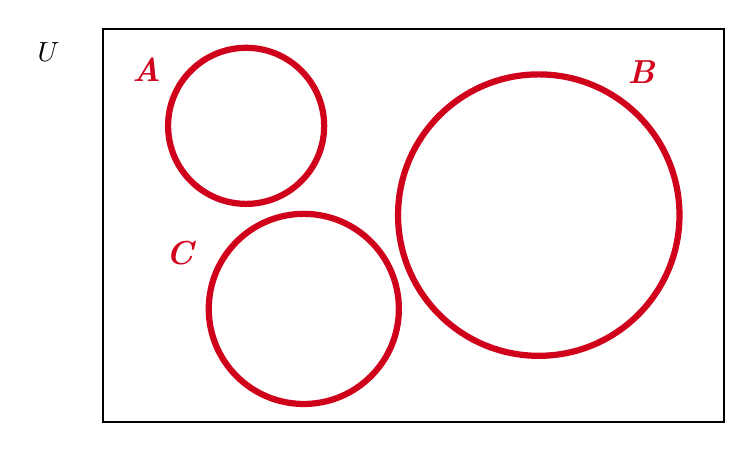
\begin{tikzpicture}[x=0.75pt,y=0.75pt,yscale=-1,xscale=1,scale = 0.8]
%uncomment if require: \path (0,256); %set diagram left start at 0, and has height of 256

%Shape: Rectangle [id:dp03257259596647377] 
\draw  [color={rgb, 255:red, 0; green, 0; blue, 0 }  ,draw opacity=1 ] (147,6) -- (521,6) -- (521,243) -- (147,243) -- cycle ;
%Shape: Circle [id:dp3347773199535533] 
\draw  [color={rgb, 255:red, 208; green, 2; blue, 27 }  ,draw opacity=1 ][line width=2.25]  (186,64.5) .. controls (186,38.54) and (207.04,17.5) .. (233,17.5) .. controls (258.96,17.5) and (280,38.54) .. (280,64.5) .. controls (280,90.46) and (258.96,111.5) .. (233,111.5) .. controls (207.04,111.5) and (186,90.46) .. (186,64.5) -- cycle ;
%Shape: Circle [id:dp49687490158652703] 
\draw  [color={rgb, 255:red, 208; green, 2; blue, 27 }  ,draw opacity=1 ][line width=2.25]  (324.5,118.25) .. controls (324.5,71.44) and (362.44,33.5) .. (409.25,33.5) .. controls (456.06,33.5) and (494,71.44) .. (494,118.25) .. controls (494,165.06) and (456.06,203) .. (409.25,203) .. controls (362.44,203) and (324.5,165.06) .. (324.5,118.25) -- cycle ;
%Shape: Circle [id:dp6548748771357666] 
\draw  [color={rgb, 255:red, 208; green, 2; blue, 27 }  ,draw opacity=1 ][line width=2.25]  (210.5,174.75) .. controls (210.5,143.13) and (236.13,117.5) .. (267.75,117.5) .. controls (299.37,117.5) and (325,143.13) .. (325,174.75) .. controls (325,206.37) and (299.37,232) .. (267.75,232) .. controls (236.13,232) and (210.5,206.37) .. (210.5,174.75) -- cycle ;

% Text Node
\draw (173,31) node [scale=1,color={rgb, 255:red, 245; green, 166; blue, 35 }  ,opacity=1 ] [align=left] {\textit{\textcolor[rgb]{0.82,0.01,0.11}{{\large \textbf{A}}}}};
% Text Node
\draw (107,16) node  [align=left] {$ $};
% Text Node
\draw (114,20) node   {$U$};
% Text Node
\draw (471,32) node [scale=1,color={rgb, 255:red, 245; green, 166; blue, 35 }  ,opacity=1 ] [align=left] {\textit{\textbf{{\large \textcolor[rgb]{0.82,0.01,0.11}{B}}}}};
% Text Node
\draw (193,141) node [scale=1,color={rgb, 255:red, 245; green, 166; blue, 35 }  ,opacity=1 ] [align=left] {{\large \textbf{\textit{\textcolor[rgb]{0.82,0.01,0.11}{C}}}}};


\end{tikzpicture}